\begin{figure}[tb]
\centering
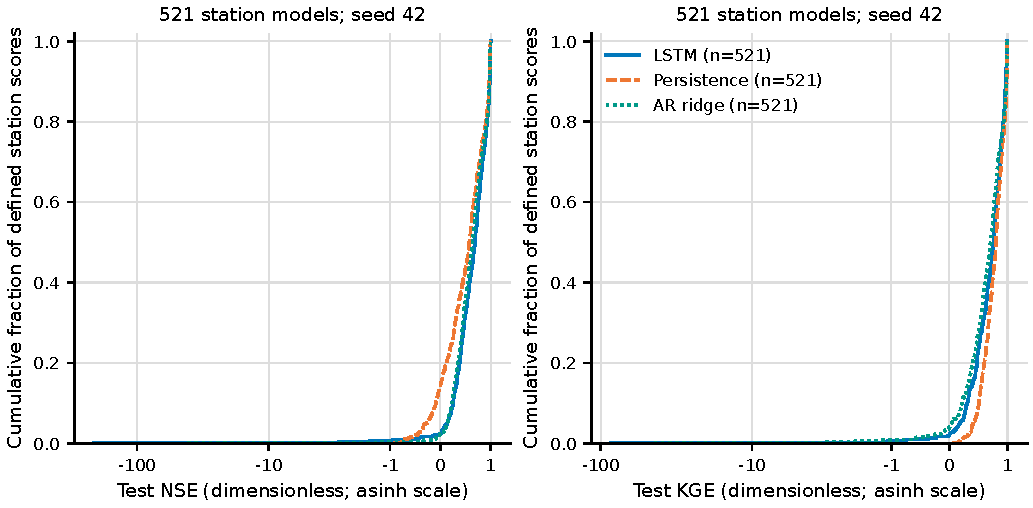
\includegraphics[width=\textwidth]{fig01_test_distribution.pdf}
\caption{Empirical distributions of test NSE and KGE across all 521 stations. Each station contributes one freshly trained, seed-42 LSTM with the same globally selected parameters. Q-history references use identical target dates. All negative results are included. An asinh horizontal scale preserves extreme negative tails.}
\end{figure}
\begin{figure}[tb]
\centering
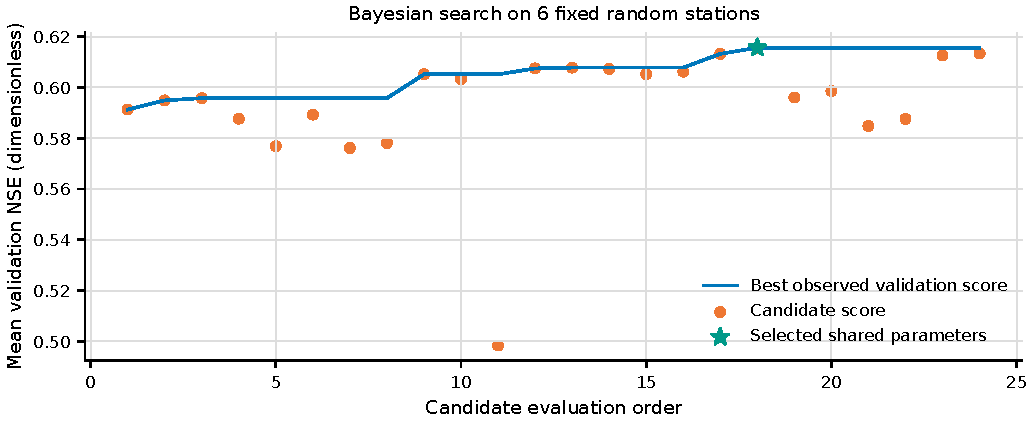
\includegraphics[width=\textwidth]{fig02_bayesian_search.pdf}
\caption{24 global configurations evaluated by the unweighted mean validation NSE on the same 6 randomly sampled stations. The first four candidates reproduce the initial grid; subsequent candidates use the seeded TPE sampler. The selected star marks the best observed validation configuration.}
\end{figure}
\begin{figure}[tb]
\centering
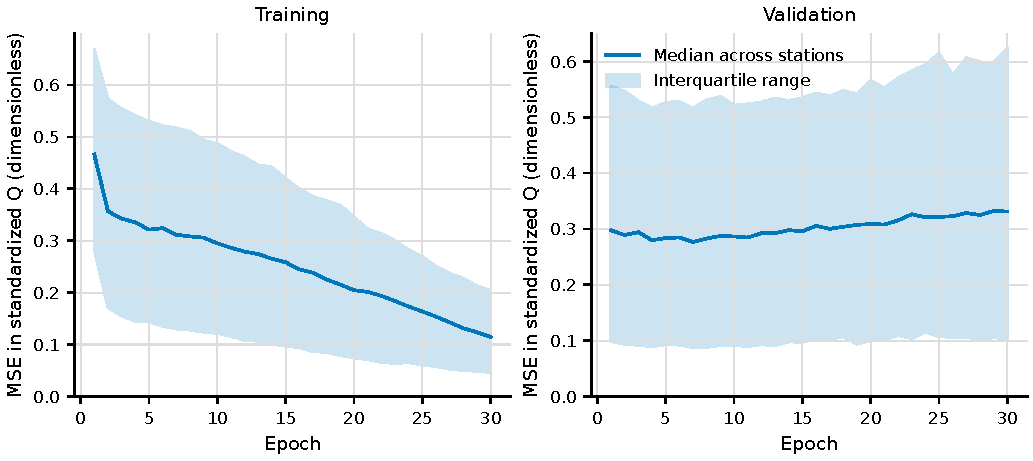
\includegraphics[width=\textwidth]{fig03_final_learning.pdf}
\caption{Final fresh-model learning curves for 521 stations sharing one configuration and seed 42. Lines show the median and shading the interquartile range across stations. Q scaling uses each station's training period only.}
\end{figure}